\chapter{Validation in Theta}
\section{Overview}
As mention: in the tetha specification.
"Theta is a generic, modular and configurable model checking framework developed at the Critical Systems Research Group of Budapest University of Technology and Economics, aiming to support the design and evaluation of abstraction refinement-based algorithms for the reachability analysis of various formalisms."
The way the Validator for witness 2.0 was implented in Theta is using XCFAs and Product Automaton. Even though 
XCFA's was chosen as formalism for further extensibility in the current version of the validator only the CFA
capabilities where used. For te moment the validator only supports Violation Witnesss. The way the violation
witness verifier works is described in the scheme below.

\begin{figure}[h]
    \centering
    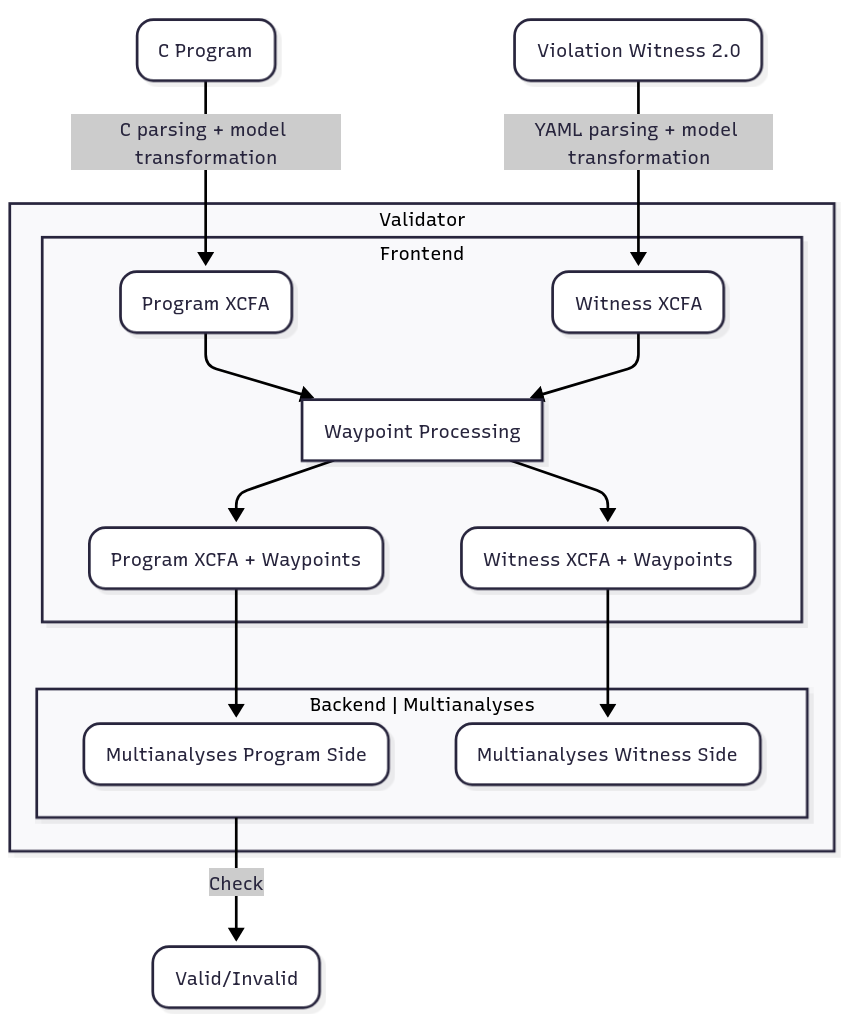
\includegraphics[width=0.8\textwidth]{figures/thetaValidator.png}
    \caption{Validation overview in Theta}
    \label{fig:Validation in Theta}
\end{figure}

% ---
% config:
%       theme: redux
% ---
% flowchart TD
%     cprogram("C Program")
%     witness("Violation Witness 2.0")
    
%     subgraph verifier["Validator"]
%         subgraph frontend["Frontend"]
%             programXCFA("Program XCFA")
%             witnessXCFA("Witness XCFA")
%             subgraph waypointProcessing["Waypoint Processing"]
%             end
%             programXCFAWay("Program XCFA + Waypoints")
%             witnessXCFAWay("Witness XCFA + Waypoints")
%         end
        
%         subgraph backend["Backend | Multianalyses"]
%             multiProgram("Multianalyses Program Side")
%             multiWitness("Multianalyses Witness Side")
%         end
%     end
    
%     output("Valid/Invalid")
    
%     cprogram -->|"C parsing + model transformation"| programXCFA
%     witness -->|"YAML parsing + model transformation"| witnessXCFA
%     programXCFA --> waypointProcessing
%     witnessXCFA --> waypointProcessing
%     waypointProcessing --> programXCFAWay
%     waypointProcessing --> witnessXCFAWay
%     programXCFAWay --> multiProgram
%     witnessXCFAWay --> multiWitness
%     backend -->|"Check"| output


There is no specification (and thus no specific safety property), because for the 
violation witness we are checking the reachability property—whether the error location
in the program and the target location in the witness are reached. The target location
of the witness is modeled as an error state to make the algorithm easy compatible with Multianalyses.

The C program is parsed and transformed into the program XCFA. The witness is parsed as YAML and 
then transformed into the witness XCFA. The violation witness can include waypoints of type avoid. 
In XCFA, a single trap node is created that all avoid waypoints point to. This works because the 
trap node (not connected to any other node) traps the execution of the violation witness, which 
means the error state of this witness cannot be reached.

While transforming the C program from AST to XCFA, much of the AST node data is added as metadata 
to the XCFA locations and edges. This metadata is used to ensure that the waypoints of the witness 
point to the correct places in the program XCFA. The pointing and correlation between the XCFAs are 
done using a global variable waypoint, which is assigned in the program XCFA and assumed in the 
witness XCFA.

From each XCFA, a Multianalysis side is created. Then the sides are combined to form the Multianalysis. 
Because of how the waypoint variable is handled, the Multianalysis is straightforward: each side 
is moved in sequence, starting from the program XCFA, until error states are reached in both XCFAs.

If both error states are reached, the witness is considered valid; otherwise, it is considered invalid.

\section{Generating XCFA from Violation Witnesses}
Within the validator in Theta, a crucial step involves transforming Violation Witnesses 
from their YAML into a more formal structure, specifically XCFA.

To facilitate this conversion, we need a clear methodology for translating each waypoint into 
its corresponding XCFA elements. Below, for every waypoint type, we'll outline how it's translated into 
the corresponding elements of the XCFA.
For our current purposes, it is sufficient to consider a waypoint (\texttt{wp}) variable as directly corresponding 
to a specific location in the C source file. The XCFA program itself also identifies these locations. 
Accordingly, each time the XCFA program arrives at one of these points, the XCFA witness
is called to process the same location. 
In our specific case, since the waypoints for the witness are essentially edges, the \texttt{wp} 
variable role is simply to determine which particular edge needs to be checked.

We consider two types of assumption waypoints:
\begin{itemize}
  \item An \textbf{avoid assumption} specifies a condition that the program must 
    \textit{not} satisfy. In other words, this assumption must not be met.
    An avoid assumption can be thought of as a negated follow assumption that 
    does not cause an advancement to the next segment.
    This implies that each time the program logic encounters an avoid assumption, 
    it must check that the specified condition does not hold.
    If the condition does not hold (i.e., the avoidance is successful), the program can 
    be modeled as having an edge transitioning back to, or remaining within, the current segment node.
    Conversely, if the condition \emph{does} hold (i.e., the program is unsuccessful in avoiding it), 
    then the execution will have no further states to transition to.
  \item A \textbf{follow assumption} dictates that the program \textit{must} 
    traverse a specific waypoint within the current segment.
    After successfully passing through this waypoint, the program is required to transition 
    to the next segment. This means the waypoint associated with a \textbf{follow} assumption 
    must be visited only once.
    Therefore, this type of assumption is represented by an edge leading from the current 
    state (after satisfying the waypoint condition) to the node representing the subsequent segment.
\end{itemize}

\begin{figure}[htbp]
  \centering
  \begin{minipage}[t]{0.35\textwidth}
    \begin{lstlisting}[style=c, columns=flexibl]
    - segment:
      - waypoint:
        type: "assumption"
        action: "avoid"
        constraint: <C_1>
        location: <wp_1>
      - waypoint:
        type: "assumption"
        action: "avoid"
        constraint: <C_2>
        location: <wp_2>
      - waypoint:
        type: "assumption"
        action: "follow"
        constraint: <C_3>
        location: <wp_3>
    \end{lstlisting}
    \end{minipage}
    \begin{tikzpicture}[
        baseline=(current bounding box.north),
        node distance=2cm,
        >={Stealth[scale=1.2]},
        every edge/.style={draw, ->},
        solidnode/.style={draw, circle, minimum size=1.2cm}, % Solid nodes
        dashednode/.style={draw, dashed, circle, minimum size=1.2cm} % Dashed nodes
    ]

    \node[dashednode] (SN1) {$s_{n-1}$};
    \node[solidnode, below=1cm of SN1] (SN) {$s_n$};
    \node[dashednode, below=1cm of SN] (SN2) {$s_{n+1}$};

    \path (SN1) edge[dashed] (SN)
        (SN) edge[out=150, in=210, min distance=1.2cm] node[left] {$\neg C_1 \land wp_1$} (SN)
        (SN) edge[out=150, in=210, min distance=4.5cm] node[left] {$\neg C_2 \land wp_2$} (SN)
        (SN) edge node[midway, right] {$C_3 \land wp_3$} (SN2); 

    \end{tikzpicture}
  \caption{XCFA mapping of the assumtion type waypoints and their constrains. The \texttt{C}
  variables are c expressions and the \texttt{wp} variables are just a tuple of row:col.}
  \label{fig:combined}
\end{figure}

A while loop provides a good example for understanding the difference between 
\emph{avoid} and \emph{follow} assumptions.
To clarify the usual confusion surrounding these concepts, and to explain why they 
are necessary and defined in this manner, consider the following illustration.
Suppose the objective is to ensure that a variable v always remains less than 256.
One could achieve this by employing a \emph{follow} assumption, such as v < 256, 
applied across n distinct program segments.
Alternatively, a more concise approach is to define a single \emph{avoid} 
assumption for the relevant segment, for instance, to avoid paths where v > 255.

\begin{figure}[htbp]
  \centering
  \begin{minipage}[t]{0.45\textwidth}
    \begin{lstlisting}[style=c]
    while (i < n) {
      v = nondet(); 
      // AVOID assume v > 255
      s += v;
      ++i;
    }
    \end{lstlisting}
  \end{minipage}
  \begin{tikzpicture}[
      baseline=(current bounding box.north),
      node distance=1.6cm,
      >={Stealth[scale=1.0]},
      every edge/.style={draw, ->},
      solidnode/.style={draw, circle, minimum size=0.8cm},
      dashednode/.style={draw, dashed, circle, minimum size=0.8cm},
      scale=1,
      transform shape
  ]

  % Nodes
  \node[solidnode] (loop_start) {$\ell_0$};
  \node[solidnode, below of=loop_start] (main_path) {$\ell_1$};
  \node[solidnode, right of=loop_start] (alternative) {$\ell_1$};

  % Incoming dashed arrow (added as requested)
  \node[left of=loop_start, xshift=-0.5cm] (incoming) {};
  \draw[dashed, ->] (incoming) -- node[above] {entry} (loop_start);

  % Transitions
  \path 
      (loop_start) edge node[right] {$i < n$} (main_path)
      (loop_start) edge node[above] {$i \geq n$} (alternative)
      (main_path) edge[bend left=50] node[left] {$\begin{array}{l}
                                   v := nondet()\\ 
                                   s := s + v\\
                                   i := i + 1
                                   \end{array}$} (loop_start);

  % Outgoing dashed arrow (added as requested)
  \node[right of=alternative, xshift=0.5cm] (outgoing) {};
  \draw[dashed, ->] (alternative) -- node[above] {exit} (outgoing);

  \end{tikzpicture}

  \caption{A Simple Whileloop and its corresponding branching in the XCFA of the program.}
  \label{fig:combined}
\end{figure}

Branching waypoints can be located at control flow statements such as \texttt{if}, \texttt{while}, a 
\texttt{ternary operator (?:)}, or a \texttt{switch} statement.
It is important to first note that in an XCFA, these C constructs are all represented as branching structures.
The XCFA representation for \texttt{if}, \texttt{while} statements and the \texttt{ternary operator (?:)} is generally 
similar, whereas it tends to be more complex for \texttt{switch} statements.
As an illustration, Figure~3.3 depicts the XCFA of a \texttt{while} loop, where the XCFA branches into two directions. 
A \texttt{switch} statement, in contrast, typically involves a greater number of branches.
This branching mechanism enables the differentiation of the path taken within the XCFA program 
solely by using the \texttt{wp} variable.
For example, if a branching waypoint indicates that the \texttt{while} loop condition evaluates to true,
the \texttt{wp} variable for that waypoint would be mapped to the edge between $\ell_0$ and $\ell_1$. 
Consequently, if the XCFA program follows the path corresponding to the condition $i>n$ (representing 
the 'true' branch in this scenario), we can determine that this specific branch was taken by inspecting 
the \texttt{wp} variable.



In the current version of Theta's validator, we only support \texttt{if} and \texttt{while} types of branching waypoints:
\begin{itemize}
  \item An \textbf{avoid branching} waypoint dictates that the program execution should never 
    traverse the branch specified by this waypoint. In other words, the \texttt{wp} variable 
    should never be equal to (i.e., point to) the location associated with this type of waypoint.
    To represent this in the witness XCFA, no specific action is taken; essentially, no edge is defined 
    for this type of waypoint. This is because encountering this type of waypoint signifies that the
    program execution should halt (i.e., "get stuck").
    This approach differs from the previously discussed \texttt{avoid assumption}. In the case of an 
    \texttt{avoid assumption}, even if the \texttt{wp} variable aligns with the waypoint's location, 
    the execution can still proceed if the associated constraint does not hold.
    However, for the type of waypoint being discussed here, encountering it mandates an immediate stop of the execution.
    This is achieved in the witness XCFA by not adding an edge, effectively meaning there is no subsequent state to transition to.
  \item A \textbf{follow branching} waypoint indicates that the program execution \emph{must} 
    follow this particular branch. We can easily verify if the program indeed followed this
    branch by checking if the \texttt{wp} variable is equal to the location of this waypoint. 
    In the witness XCFA, this can be represented by an edge leading to the subsequent segment, which is
    traversed if the \texttt{wp} variable matches this waypoint's location.
\end{itemize}

It should be noted that branching waypoints possess a constraint indicating how the condition of an \texttt{if}, \texttt{while}, 
\texttt{ternary operator (?:)}, or \texttt{switch} statement evaluated.
For \texttt{if}, \texttt{while}, and the \texttt{ternary operator (?:)}, this evaluation can result in "true" or "false".
For a \texttt{switch} statement, it can be an integer constant (representing the value of the variable being switched upon) or the "default" case.
Consequently, this constraint informs us which path the program should take.
Since the \texttt{wp} variable is associated with the path we intend the program to follow, this implies that the \texttt{wp}
variable also implicitly "contains" this constraint (i.e., the constraint can be inferred from it).
Therefore, in a potentially simplified YAML witness representation (such as one discussed below), the explicit constraint might 
be omitted, with only the location being kept. This, however, is not the case in the complete or actual YAML witness specification.


\begin{figure}[H]
  \centering
  \begin{minipage}[t]{0.35\textwidth}
    \begin{lstlisting}[style=c, columns=flexibl]
    - segment:
      - waypoint:
        type: "branching"
        action: "avoid"
        location: <wp_1>
      - waypoint:
        type: "branching"
        action: "avoid"
        location: <wp_2>
      - waypoint:
        type: "branching"
        action: "follow"
        location: <wp_3>
    \end{lstlisting}
    \end{minipage}
    \hspace{2cm}
    \begin{tikzpicture}[
        baseline=(current bounding box.north),
        node distance=2cm,
        >={Stealth[scale=1.2]},
        every edge/.style={draw, ->},
        solidnode/.style={draw, circle, minimum size=1.2cm}, % Solid nodes
        dashednode/.style={draw, dashed, circle, minimum size=1.2cm} % Dashed nodes
    ]

    \node[dashednode] (SN1) {$s_{n-1}$};
    \node[solidnode, below=1cm of SN1] (SN) {$s_n$};
    \node[dashednode, below=1cm of SN] (SN2) {$s_{n+1}$};

    \path (SN1) edge[dashed] (SN)
        (SN) edge node[midway, right] {$wp_3$} (SN2); 

    \end{tikzpicture}
  \caption{XCFA mapping of a branching-type waypoint, where the \texttt{wp} variable is a tuple (row:col, constraint)
  indicating which XCFA branch was taken.}
  \label{fig:combined}
\end{figure}

There is only one type of target waypoint:
\begin{itemize}
  \item A \textbf{follow target} waypoint indicates that the program execution should reach 
    the designated error location. It is positioned immediately before the error, 
    ensuring that no other program evaluations occur before the error state is encountered. 
    In the witness XCFA, this can be readily represented by an edge pointing directly to the error location.
\end{itemize}
This type of waypoint does not have an associated constraint.

\begin{figure}[htbp]
  \centering
  \begin{minipage}[t]{0.35\textwidth}
    \begin{lstlisting}[style=c, columns=flexibl]
    - segment:
      - waypoint:
        type: "target"
        action: "follow"
        location: <wp_0>
    \end{lstlisting}
    \end{minipage}
    \hspace{2cm}
    \begin{tikzpicture}[
        baseline=(current bounding box.north),
        node distance=2cm,
        >={Stealth[scale=1.2]},
        every edge/.style={draw, ->},
        solidnode/.style={draw, circle, minimum size=1.2cm}, % Solid nodes
        dashednode/.style={draw, dashed, circle, minimum size=1.2cm} % Dashed nodes
    ]

    \node[dashednode] (SN1) {$s_{n-1}$};
    \node[solidnode, below=1cm of SN1] (SN) {$s_n$};
    \node[dashednode, below=1cm of SN] (SN2) {error};

    \path (SN1) edge[dashed] (SN)
        (SN) edge node[midway, right] {$wp_0$} (SN2); 

    \end{tikzpicture}
  \caption{XCFA mapping of target type waypoint. The \texttt{wp} variables are a tuple of row:col.}
  \label{fig:combined}
\end{figure}


The following is an example segment that includes all the aforementioned types of waypoints.

\begin{figure}[H]
  \centering
  \begin{minipage}[t]{0.35\textwidth}
    \begin{lstlisting}[style=c, columns=flexibl]
    - segment:
      - waypoint:
        type: "branching"
        action: "avoid"
        location: <wp_1>
      - waypoint:
        type: "assumption"
        action: "avoid"
        constraint: <C_2>
        location: <wp_2>
      - waypoint:
        type: "target"
        action: "follow"
        location: <wp_3>
    \end{lstlisting}
    \end{minipage}
    \begin{tikzpicture}[
        baseline=(current bounding box.north),
        node distance=2cm,
        >={Stealth[scale=1.2]},
        every edge/.style={draw, ->},
        solidnode/.style={draw, circle, minimum size=1.2cm}, % Solid nodes
        dashednode/.style={draw, dashed, circle, minimum size=1.2cm} % Dashed nodes
    ]

    \node[dashednode] (SN1) {$s_{n-1}$};
    \node[solidnode, below=1cm of SN1] (SN) {$s_n$};
    \node[dashednode, below=1cm of SN] (SN2) {$s_{n+1}$};

    \path (SN1) edge[dashed] (SN)
        (SN) edge[out=150, in=210, min distance=1.2cm] node[left] {$\neg C_2 \land wp_2$} (SN)
        (SN) edge node[midway, right] {$wp_3$} (SN2); 

    \end{tikzpicture}
  \caption{XCFA mapping of a final segment containing branching, assumption, and target waypoints, along with their respective constraints.}
  \label{fig:combined}
\end{figure}

A segment is designated as final if its follow waypoint is a target.

\section{Example}
To clarify how the validator works, we provide a detailed example of its execution.
Displayed below is an unsafe program, accompanied by its corresponding violation witness.

\begin{lstlisting}[style=c,caption=C Program,label=lst:code]
int main() {
  unsigned char n = nondet();
  if (n == 0) return 0;
  
  unsigned char v = 0;
  unsigned char s = 0;
  unsigned int i = 0;
  
  while (i < n) {
    v = nondet();
    s += v;
    ++i;
  }
  
  if (s < v) { reach_error(); return 1; }
  if (s > 65025) { reach_error(); return 1; }
  
  return 0;
}
\end{lstlisting}

\begin{lstlisting}[style=yaml, language=C,caption=Violation Witness]
- entry_type: "violation_sequence"
metadata: <...>
content:
add n here
- segment: 
  - waypoint:
    type: "branching"
    action: "follow"
    constraint: "false"
    location: 11:3
- segment: 
  - waypoint:
    type: "assumption"
    action: "follow"
    constraint: "v == 0"
    location: 15:3
- segment:
  - waypoint:
    type: "assumption"
    action: "follow"
    constraint: "s == 0"
    location: 16:3
- segment:
  - waypoint:
    type: "branching"
    action: "follow"
    constraint: "true"
    location: 17:3
- segment:
  - waypoint:
    type: "target"
    action: "follow"
    location: 23:3
\end{lstlisting}

Unfortunetily, the XCFA of the program is quite complex and holds quite large amounts of information.
Therefore here we are going to work with a simplied version of the program XCFA.

Take ti from digrapth put it on mermaid and simplify bothe winesses

Here is the witness:

Here are the witness after the waypoint are mached
Here show both XCFAs and show the code in between pointing wher the witnesses are pointing

Explain hwo the the XCFAs would be executed one after each other.

\section{Theta's Validation Capabilities Compared to Other Verification Tools}
